\razdelek{Teorija odločanja}

\begin{naloga}{?}{Vaje OR 30.3.2016}
\begin{vprasanje}
Na ulici nas ustavi neznanec in nam predlaga met kovanca.
Če pade grb, nam izplača $250000 €$,
če pade glava, pa mi njemu $100000 €$.
Ali naj sprejmemo ponudbo?
\end{vprasanje}

\begin{odgovor}
Če predpostavimo, da je kovanec pošten,
je potem pričakovani dobiček ob metu kovanca enak
$$
{1 \over 2} \cdot 250000 € - {1 \over 2} \cdot 100000 € = 75000 € .
$$
Ta vrednost je večja od ničelnega dobička, če ponudbe ne sprejmemo,
zato se nam izplača ponudbo sprejeti.
Seveda gre pri tej odločitvi tudi za oceno,
kolikšno tveganje smo pripravljeni sprejeti
-- ali si lahko privoščimo izgubiti $100000 €$, če ne bomo imeli sreče?
\end{odgovor}
\end{naloga}


\begin{naloga}{Batagelj, Kaufman}{\cite[Naloga~4.2]{bk}}
\begin{vprasanje}
Trgovina pri pekarni kupuje žemlje po $0.2 €$
in jih prodaja po $0.4 €$.
Skozi leta poslovanja so izračunali naslednjo porazdelitev za prodajo žemljic.
\begin{center}
\begin{tabular}{c|cccccc}
Prodaja & $50$ & $60$ & $70$ & $80$ & $90$ & $100$ \\
\hline
Verjetnost & $0.1$ & $0.15$ & $0.3$ & $0.2$ & $0.15$ & $0.1$
\end{tabular}
\end{center}
Če žemelj zmanjka, naročijo pri pekarni razliko,
pri čemer jih žemlja tedaj stane $0.3 €$.
Ob koncu dneva jim pekarna odkupi presežek po $0.15 €$ na žemljo.
Koliko žemelj se trgovini splača kupiti?
\end{vprasanje}

\begin{odgovor}
Naj bo $x$ število kupljenih žemelj, $k$ pa število prodanih žemelj.
Če je $k \le x$, imamo dobiček
$$
k \cdot 0.2 € - (x-k) \cdot 0.05 € = k \cdot 0.25 € - x \cdot 0.05 € .
$$
Če pa je $k \ge x$, je dobiček enak
$$
x \cdot 0.2 € + (k-x) \cdot 0.1 € = k \cdot 0.1 € + x \cdot 0.1 € .
$$
Pri $x = k$ obe formuli dasta dobiček $k \cdot 0.2 €$.
Izračunajmo pričakovani dobiček pri naročilu $x$ žemelj za različne intervale:
\begin{align*}
x \le 50:         &\ x \cdot 0.1 € +
                     (0.1 \cdot 50 + 0.15 \cdot 60 + 0.3 \cdot 70 \ + \\
                  &\  0.2 \cdot 80 + 0.15 \cdot 90 + 0.1 \cdot 100)
                     \cdot 0.1 € \\
                  &= x \cdot 0.1 € + 7.45 € \\
50 \le x \le 60:  &\ x \cdot (0.9 \cdot 0.1 € - 0.1 \cdot 0.05 €) +
                     0.1 \cdot 50 \cdot 0.25 € \ + \\
                  &\ (0.15 \cdot 60 + 0.3 \cdot 70 + 0.2 \cdot 80 +
                      0.15 \cdot 90 + 0.1 \cdot 100) \cdot 0.1 € \\
                  &= x \cdot 0.085 € + 8.2 € \\
60 \le x \le 70:  &\ x \cdot (0.75 \cdot 0.1 € - 0.25 \cdot 0.05 €) +
                     (0.1 \cdot 50 + 0.15 \cdot 60) \cdot 0.25 € \ + \\
                  &\ (0.3 \cdot 70 + 0.2 \cdot 80 + 0.15 \cdot 90 +
                      0.1 \cdot 100) \cdot 0.1 € \\
                  &=  x \cdot 0.0625 € + 9.55 € \\
70 \le x \le 80:  &\ x \cdot (0.45 \cdot 0.1 € - 0.55 \cdot 0.05 €) +
                     (0.1 \cdot 50 + 0.15 \cdot 60 \ + \\
                  &\ 0.3 \cdot 70) \cdot 0.25 € +
                     (0.2 \cdot 80 + 0.15 \cdot 90 + 0.1 \cdot 100)
                     \cdot 0.1 € \\
                  &= x \cdot 0.0175 € + 12.7 € \\
80 \le x \le 90:  &\ x \cdot (0.25 \cdot 0.1 € - 0.75 \cdot 0.05 €) +
                     (0.1 \cdot 50 + 0.15 \cdot 60 + 0.3 \cdot 70 \ + \\
                  &\  0.2 \cdot 80) \cdot 0.25 € +
                     (0.15 \cdot 90 + 0.1 \cdot 100) \cdot 0.1 € \\
                  &= -x \cdot 0.0125 € + 15.1 € \\
90 \le x \le 100: &\ x \cdot (0.1 \cdot 0.1 € - 0.9 \cdot 0.05 €) +
                     (0.1 \cdot 50 + 0.15 \cdot 60 + 0.3 \cdot 70 \ + \\
                  &\  0.2 \cdot 80 + 0.15 \cdot 90) \cdot 0.25 € +
                     0.1 \cdot 100 \cdot 0.1 € \\
                  &= -x \cdot 0.035 € + 17.125 € \\
x \ge 100:        &\ -x \cdot 0.05 € +
                     (0.1 \cdot 50 + 0.15 \cdot 60 + 0.3 \cdot 70 \ + \\
                  &\  0.2 \cdot 80 + 0.15 \cdot 90 + 0.1 \cdot 100)
                     \cdot 0.25 € \\
                  &= -x \cdot 0.05 € + 18.625 €
\end{align*}
Funkcija pričakovanega dobička je torej zvezna in odsekoma linearna v $x$,
pri čemer je smerni koeficient pozitiven pri $x < 80$
in negativen pri $x > 80$.
Pričakovan dobiček torej maksimiziramo pri naročilu $80$ žemelj
-- tedaj ta znaša
$$
80 \cdot 0.0175 € + 12.7 € = 14.1 € .
$$
\end{odgovor}
\end{naloga}


\begin{naloga}{?}{Izpit OR 5.6.2014}
\begin{vprasanje}[operacija]
Pacient ima na voljo operacijo.
Brez operacije bo živel natanko $3$ mesece.
Z uspeš\-no opravljeno operacijo bo živel natanko $12$ mesecev.
Operacija je neuspešna z verjetnostjo $0.3$
(v tem primeru pacient dočaka $0$ mesecev).
Cilj pacienta je maksimiranje pričakovane življenjske dobe.
\begin{enumerate}[(a)]
\item Ali naj pacient sprejme operacijo?
\item Pacient lahko opravi predhodni test,
ki z zanesljivostjo $0.9$ napove uspeš\-nost operacije,
vendar z verjetnostjo $0.005$ pacient zaradi komplikacij med testom umre.
Ali naj pacient opravi test?
\end{enumerate}
Nariši odločitveno drevo
in odločitve sprejmi na podlagi izračunanih ve\-rjet\-no\-sti!
\end{vprasanje}

\begin{odgovor}
\begin{enumerate}[(a)]
\item Ob opravljeni operaciji
je pričakovana življenjska doba (v mesecih) enaka
$$
0.7 \cdot 12 + 0.3 \cdot 0 = 8.4 .
$$
Ker je to več od $3$ mesecev brez operacije, se zanjo pacient odloči.

\item Zanesljivost $0.9$ razumemo tako,
da test z verjetnostjo $0.9$ pravilno napove vsak izid operacije,
torej
\begin{align*}
P(\text{test napove uspeh} \;|\; \text{operacija je uspešna}) &= 0.9
\quad \text{in} \\
P(\text{test napove uspeh} \;|\; \text{operacija je neuspešna}) &= 0.1 .
\end{align*}
Izračunajmo še verjetnosti napovedi testa
ter uspešnosti operacije ob vsaki napovedi.
\begin{small}
\begin{align*}
P(\text{test napove uspeh}) &= 0.7 \cdot 0.9 + 0.3 \cdot 0.1 = 0.66 \\
P(\text{test napove neuspeh}) &= 0.7 \cdot 0.1 + 0.3 \cdot 0.9 = 0.34 \\
P(\text{operacija je uspešna} \;|\; \text{test napove uspeh})
&= {0.7 \cdot 0.9 \over 0.66} = {21 \over 22} \approx 0.9545 \\
P(\text{operacija je neuspešna} \;|\; \text{test napove uspeh})
&= {0.3 \cdot 0.1 \over 0.66} = {1 \over 22} \approx 0.0455 \\
P(\text{operacija je uspešna} \;|\; \text{test napove neuspeh})
&= {0.7 \cdot 0.1 \over 0.34} = {7 \over 34} \approx 0.2059 \\
P(\text{operacija je uspešna} \;|\; \text{test napove neuspeh})
&= {0.3 \cdot 0.9 \over 0.34} = {27 \over 34} \approx 0.7941
\end{align*}
\end{small}
Ob upoštevanju, da se bo test končal brez komplikacij z verjetnostjo $0.995$,
sta verjetnosti pozitivnega in negativnega izida testa brez komplikacij
enaki $0.6567$ oziroma $0.3383$.

S pomočjo zgoraj izračunanih verjetnosti
lahko narišemo odločitveno drevo s slike~\fig{}.
Izračunamo lahko, da je ob opravljanju testa
pričakovana življenjska doba $8.537$ mesecev,
kar je več kot $8.4$ mesecev brez testa,
zato se odločimo za test.
Če test napove uspeh, se odločimo za operacijo, sicer pa ne.
\end{enumerate}

\begin{slika}
\makebox[\textwidth][c]{
\pgfslika
}
\podnaslov{Odločitveno drevo}
\end{slika}
\end{odgovor}
\end{naloga}


\begin{naloga}{?}{Vaje OR 30.3.2016}
\begin{vprasanje}
Podjetje je razvilo produkt,
za katerega je konkurenca pripravljena plačati $15 \ME$.
Če se odločijo samostojno prodajati produkt,
jih vzpostavitev proizvodnje stane $6 \ME$,
za vsak uspešno prodan produkt pa dobijo $600 €$.
Računajo, da bi z ve\-rjet\-nost\-jo $0.5$ investicija uspela
in bi prodali $100000$ produktov,
z verjetnostjo $0.5$ pa bi projekt propadel
in bi prodali zgolj $10000$ produktov.
Podjetje se lahko odloči tudi za neodvisno raziskavo trga.
Ta stane $1 \ME$,
z verjetnostjo $2/3$ pa bo pravilno napovedala uspeh projekta
(ne glede na to, ali bi ta uspel ali ne).
Kako naj se podjetje odloči?

\end{vprasanje}
\begin{odgovor}
\end{odgovor}
\end{naloga}


\begin{naloga}{?}{Izpit OR 24.6.2015}
\begin{vprasanje}
Veliki koncert skupine FiM
se bo odvijal v dvorani s $100$ neoznačenimi sedeži.
Prireditelj se lahko odloči, da proda $100$, $101$, $102$ ali $103$ karte
(povpraševanja je dovolj).
Znane so verjetnosti $p_0 = 0.2$, $p_1 = 0.3$, $p_2 = 0.4$ in $p_3 = 0.1$,
kjer je $p_i$ verjetnost, da $i$ kupcev kart ne pride na koncert
(ne glede na število prodanih kart).
Vsaka prodana karta prinese $10 €$ dobička,
vsak obiskovalec, ki ne bo mogel v dvorano, pa pomeni $30 €$ stroškov
(ker je že plačal $10 €$ za karto, ima torej organizator $20 €$ izgube).
Koliko kart naj prireditelj proda, da bo pričakovani dobiček čim večji?

\end{vprasanje}
\begin{odgovor}
\end{odgovor}
\end{naloga}


\begin{naloga}{?}{Kolokvij OR 31.5.2012}
\begin{vprasanje}
Rexhep Bajrami bi se rad naslednja štiri leta
ukvarjal s prodajo sadja in zelenjave
(po štirih letih mu poteče delovna viza).
Rad bi najel parcelo za stojnico, ki bo stala $6000 €$.
Če je lokacija dobra, bo imel $12000 €$ dobička,
če pa je lokacija slaba, bo imel le $3000 €$ dobička.
Ocenjuje, da je z verjetnostjo $2/3$ lokacija dobra,
z verjetnostjo $1/3$ pa slaba.
\begin{enumerate}[(a)]
\item Z odločitvenim drevesom opiši njegove možnosti in ugotovi,
kako naj se odloči ter kakšen dobiček naj pričakuje.
\item Za nasvet lahko vpraša znanca Seada, ki ``ima nos'' za tovrstne posle.
Sead mu lahko da nasvet, a zanj zahteva $1200 €$.
Dobro je znano, da ima Sead naslednje pogojne verjetnosti
$P(\text{Seadovo mnenje} \; | \; \text{kakovost parcele})$:
\begin{center}
\begin{tabular}{c|cc}
& dobra & slaba \\
\hline
priporoča & $2/3$ & $1/2$ \\
odsvetuje & $1/3$ & $1/2$
\end{tabular}
\end{center}
Ali naj vpraša Seada za nasvet?
Kakšen je pričakovani dobiček?
\end{enumerate}
\end{vprasanje}
\begin{odgovor}
\end{odgovor}
\end{naloga}


\begin{naloga}{Sergio Cabello}{Izpit OR 15.3.2017}
\begin{vprasanje}[dectree]
Imaš odločitveno drevo s slike~\fig{},
a nisi prepričan glede vrednosti $p \in [0, 1/3]$.
Pričakovano vrednost želiš maksimizirati.
Poišči optimalne odločitve glede na vrednost $p$.

\begin{slika}
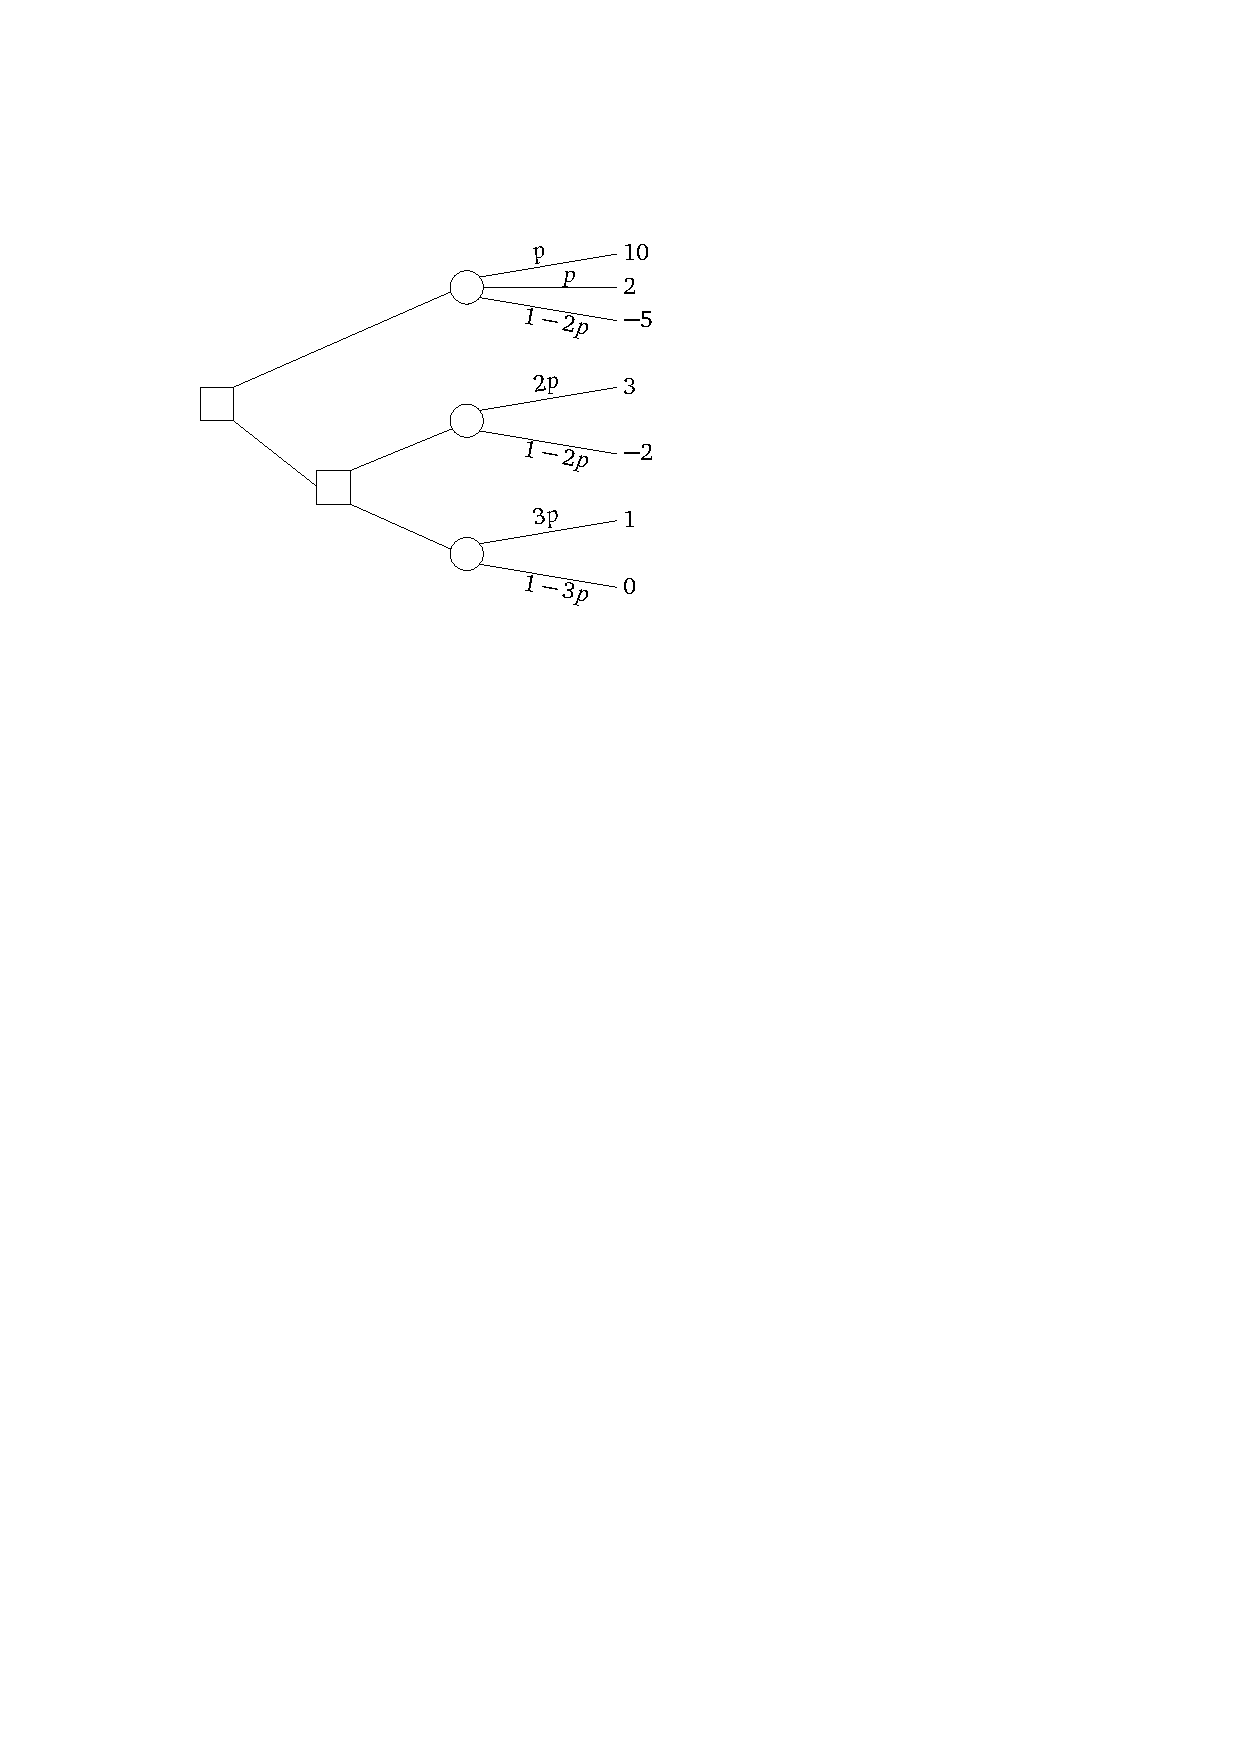
\includegraphics{slike/decision-tree.pdf}
\podnaslov{Odločitveno drevo}
\end{slika}
\end{vprasanje}
\begin{odgovor}
\end{odgovor}
\end{naloga}


\begin{naloga}{Janoš Vidali}{Izpit OR 15.12.2016}
\begin{vprasanje}[avtobus]
Mudi se ti na izpit, a ravno v trenutku,
ko prideš na postajo Konzorcij, odpelje avtobus številka 1.
Na prikazovalniku se izpiše,
da bo naslednji avtobus številka 1 prispel čez $10$ minut,
naslednji avtobus številka 6 čez $6$ minut,
naslednji avtobus številka 14 pa čez $2$ minuti.

Avtobusa 1 in 6 ob ugodnih semaforjih potrebujeta $6$ minut do postaje pri FE,
pri čemer se lahko čas vož\-nje zaradi rdeče luči na semaforju pri FF
podaljša za $1$ minuto.
Verjetnosti, da bo rdečo luč imel avtobus 1, da bo rdečo luč imel avtobus 6,
ter da bosta oba avtobusa imela zeleno luč, so enake $1/3$
(zaradi majhnega razmaka se ne more zgoditi,
da bi oba avtobusa naletela na rdečo luč).
Avtobus številka 1 nadaljuje pot do postaje pri FMF,
za kar potrebuje še $2$ minuti.

Avtobus številka 14 potrebuje $5$ minut do postaje pri študentskih domovih,
od tam pa greš peš do postaje pri FE, za kar potrebuješ še $4$ minute.
Pri tem prečkaš že\-lez\-ni\-co -- če mimo pripelje vlak
(kar se zgodi z verjetnostjo $0.05$),
se čas hoje podaljša za $3$ minute.
Ko prideš na postajo pri FE
(ne glede na to, ali si prišel z avtobusom 6 ali 14),
te čakajo še $4$ minute hoje do FMF,
vendar moraš najprej prečkati Tržaško cesto.
Če je na semaforju rdeča luč
(kar se zgodi z verjetnostjo 0.9, neodvisno od drugih dogodkov),
se lahko odločiš, da $2$ minuti počakaš na zeleno luč in potem nadaljuješ peš,
ali pa da greš nazaj do postaje in počakaš na avtobus številka $1$
(ki bo, tako kot prej, vozil še $2$ minuti do FMF).

Kakšne bodo tvoje odločitve,
da bo pričakovano trajanje poti do FMF čim krajše?
Nariši od\-lo\-čit\-ve\-no drevo
in odločitve sprejmi na podlagi izračunanih verjetnosti!
Glej sliko~\fig{} za shemo možnih poti.

\begin{slika}
\pgfslika
\podnaslov{Shema možnih poti}
\end{slika}
\end{vprasanje}
\begin{odgovor}
\end{odgovor}
\end{naloga}


\begin{naloga}{Janoš Vidali}{Izpit OR 31.1.2017}
\begin{vprasanje}
Dve podjetji bosta predstavili konkurenčna izdelka.
Možnost imaš kupiti delnice prvega podjetja za ceno $10000 €$
ali delnice drugega podjetja po ceni $5000 €$,
lahko pa se seveda odločiš tudi, da delnic ne kupiš.
Ocenjuješ, da bo z verjetnostjo $0.4$ uspelo prvo podjetje,
z verjetnostjo $0.1$ bo uspelo drugo podjetje,
z verjetnostjo $0.5$ pa ne bo uspelo nobeno izmed njiju
(ne more se zgoditi, da bi obe uspeli).
Ob uspehu prvega podjetja se bo vrednost njihovih delnic potrojila,
ob uspehu drugega podjetja pa se bo vrednost njihovih delnic popeterila
-- če si lastiš delnice uspešnega podjetja, jih torej lahko prodaš,
pri čemer bo torej dobiček enak
dvakratniku oziroma štirikratniku vloženega zneska.
Delnic neuspešnega podjetja ne bo želel nihče kupiti,
tako da je v tem primeru vloženi znesek izgubljen.

Za mnenje lahko povprašaš tržnega izvedenca,
ki bo po opravljeni raziskavi povedal,
katero od dveh podjetij ima večje možnosti za uspeh.
Če bo uspešno prvo podjetje, bo to pravilno napovedal z verjetnostjo $0.8$,
če pa bo uspešno drugo podjetje,
bo to pravilno napovedal z verjetnostjo $0.7$.
V primeru, ko podjetji ne bosta uspeli,
bo z verjetnostjo $0.4$ večje možnosti pripisal prvemu,
z verjetnostjo $0.6$ pa drugemu podjetju.
Za svoje mnenje izvedenec računa $1000 €$.

Kakšne bodo tvoje odločitve,
da bo tvoj pričakovani dobiček po odprodaji delnic čim večji?
Nariši od\-lo\-čit\-ve\-no drevo
in odločitve sprejmi na podlagi izračunanih verjetnosti.
Pričakovani dobiček tudi izračunaj.
\end{vprasanje}
\begin{odgovor}
\end{odgovor}
\end{naloga}


\begin{naloga}{Janoš Vidali}{Izpit OR 10.7.2017}
\begin{vprasanje}
Proti računalniškemu programu igraš Texas hold 'em poker.
Pravila igre tukaj niso pomembna.
Ker imaš dostop do kode programa, poznaš logiko, po kateri se ravna.
V trenutni igri si vložil $30$ žetonov, enako tudi nasprotnik.
Nasprotnik z verjetnostjo $0.6$ meni, da so odprte karte ugodnejše zate,
z verjetnostjo $0.4$ pa, da so ugodnejše zanj
(sam si ne ustvariš nobenega mnenja).
V prvem primeru je verjetnost, da so dejansko tvoje karte boljše, enaka $0.8$,
v drugem pa le $0.1$.

Nasprotnik se bo sedaj odločil, ali naj vloži še $10$ žetonov.
Sam se lahko nato odločiš, ali boš vložil $0$, $10$ ali $20$ žetonov
(skupni vložek bo torej $30$, $40$ ali $50$ žetonov).
Če je tvoj vložek manjši od nasprotnikovega,
je igra izgubljena in izgubiš do sedaj vloženo.
Če je tvoj vložek enak na\-sprot\-ni\-ko\-ve\-mu,
z nasprotnikom pogledata karte in tako določita zmagovalca.
Če je tvoj vložek višji od nasprotnikovega,
ima ta možnost odstopiti (tako pridobiš nasprotnikov vložek),
ali pa izenačiti, nakar se zmagovalec določi na podlagi kart.
Če zmagaš, pridobiš nasprotnikov vložek,
če izgubiš, pa izgubiš svojega.

V spodnji tabeli so zbrane verjetnosti dogodkov
v odvisnosti od nasprotnikovega mnenja glede kart.
Verjetnosti navedenih dogodkov pri istem mnenju so med seboj neodvisne.
\begin{center}
\makebox[\textwidth][c]{
\begin{small}
\begin{tabular}{r|cc}
dogodek $\setminus$ nasprotnikovo mnenje
& ugodnejše karte zate & za nasprotnika \\ \hline
dejansko imaš boljše karte & 0.8 & 0.1 \\
nasprotnik vloži $10$ žetonov po razkritju karte & 0.3 & 0.8 \\
nasprotnik izenači skupni vložek $40$ žetonov & 0.2 & 0.7 \\
nasprotnik izenači skupni vložek $50$ žetonov & 0.1 & 0.8
\end{tabular}
\end{small}
}
\end{center}
Na primer:
\begin{multline*}
\Pr[\text{nasprotnik izenači skupni vložek $40$ žetonov} \ | \\
| \ \text{nasprotnikovo mnenje je ``ugodnejše karte zate''}] = 0.2 .
\end{multline*}

Kakšne bodo tvoje odločitve,
da bo tvoj pričakovani dobiček po koncu igre čim večji?
Nariši odločitveno drevo
in odločitve sprejmi na podlagi izračunanih verjetnosti.
Pričakovani dobiček tudi izračunaj.
\end{vprasanje}
\begin{odgovor}
\end{odgovor}
\end{naloga}


\begin{naloga}{Janoš Vidali}{Izpit OR 29.8.2017}
\begin{vprasanje}[dectree2]
Dano je odločitveno drevo s slike~\fig{},
pri čemer velja $0 \le p \le 1/4$.
Pričakovano vred\-nost želimo maksimizirati.
Poišči optimalne odločitve in pričakovano vrednost
v odvisnosti od vrednosti parametra $p$.

\begin{slika}
\pgfslika
\podnaslov{Odločitveno drevo}
\end{slika}
\end{vprasanje}
\begin{odgovor}
\end{odgovor}
\end{naloga}


\begin{naloga}{Janoš Vidali}{Kolokvij OR 23.4.2018}
\begin{vprasanje}
Mladi podjetnik je razvil inovativen izdelek
in se odloča za nadaljnje korake pri njegovem trženju.
Naenkrat lahko naroči izdelavo $500$ izdelkov po ceni $10000 €$
ali $1000$ izdelkov po ceni $18000 €$,
lahko se pa odloči tudi, da izdelave ne naroči.
Podjetnik ocenjuje, da je izdelek tržno zanimiv z verjetnostjo $0.8$.
Odloča se, ali naj posamezen izdelek prodaja po ceni $50 €$ ali $60 €$,
pri čemer so v spodnji tabeli zbrana pričakovana števila prodanih kosov
v odvisnosti od teh pogojev.

\begin{center}
\begin{tabular}{c|cc}
& cena $50 €$ & cena $60 €$ \\
\hline
tržno zanimiv & $650$ & $550$ \\
tržno nezanimiv & $250$ & $100$ \\
\end{tabular}
\end{center}

Predpostavi, da se bodo prodali vsi izdelani kosi,
če je število teh manjše od pričakovane prodaje pri danih pogojih.

\begin{enumerate}[(a)]
\item Kako naj se podjetnik odloči, da bo pričakovani zaslužek čim večji?
Nariši od\-lo\-čit\-ve\-no drevo in ga uporabi pri sprejemanju odločitev.

\item V zadnjem trenutku je podjetnik izvedel,
da bo Podjetniški pospeševalnik objavil
razpis za nagrado za najboljši izdelek.
Razpisni pogoji zahtevajo,
da se za potrebo kontrole kvalitete izdela vsaj $1000$ izdelkov,
od katerih komisija izbere $20$ za dejansko kontrolo,
z ostalimi pa lahko prijavitelj prosto razpolaga.
Če podjetnik zmaga, bo dobil nagrado v višini $k$ evrov,
pri čemer $k \in [1000, 5000]$ še ni znan,
poleg tega pa si obeta tudi $20\%$ povečanje
pričakovanega števila prodanih kosov (v vseh zgoraj omenjenih pogojih).
Če ne zmaga, se pričakovanja ne spremenijo.
Podjetnik ocenjuje, da je verjetnost zmage enaka $0.6$,
če je izdelek tržno zanimiv,
in $0.1$, če izdelek ni tržno zanimiv.

Naj se podjetnik prijavi na razpis?
Nariši odločitveno drevo in odločitve sprejmi v odvisnosti od parametra $k$!
\end{enumerate}
\end{vprasanje}
\begin{odgovor}
\end{odgovor}
\end{naloga}


\begin{naloga}{Janoš Vidali}{Izpit OR 11.6.2018}
\begin{vprasanje}[vrac]
Podajamo se na pot v mesto na drugi strani gorovja.
Lahko se odločimo za pot po cesti okoli gorovja,
za kar bomo porabili $12$ ur.
Vendar pa nas najkrajša pot vodi čez prelaz,
ki je eno uro stran od začetne lokacije.
Žal pa so razmere v gorah nepredvidljive:
ocenjujemo, da bo z verjetnostjo $0.2$ prelaz čist
in ga bomo lahko prevozili v $5$ urah,
z ve\-rjet\-nost\-jo $0.1$ bo delno zasnežen in ga bomo prevozili v $9$ urah,
z verjetnostjo $0.7$ pa bo neprevozen,
zaradi česar se bomo morali vrniti na začetek in iti okoli gorovja
(skupno trajanje poti bo v tem primeru torej $14$ ur).

Edini, ki nam lahko kakorkoli pomaga pri oceni vremenskih razmer na prelazu,
je lokalni vrač,
ki pa živi v dolini pod goro in ne uporablja sodobne tehnologije,
s katero bi ga lahko kontaktirali.
Rade volje pa nam bo povedal, ali na gori vlada mir,
če se na poti do prelaza ustavimo pri njem.
Pogojne verjetnosti njegovega odgovora v odvisnosti od razmer na prelazu
so podane v spodnji tabeli.
\begin{center}
\makebox[\textwidth][c]{
\begin{tabular}{c|ccc}
$P\left(\text{vračev odgovor} \;\middle|\; \text{razmere na prelazu}\right)$
& čist & delno zasnežen & neprevozen \\ \hline
na gori vlada mir & $0.9$ & $0.5$ & $0.1$ \\
na gori divja vojna & $0.1$ & $0.5$ & $0.9$
\end{tabular}
}
\end{center}
Do vrača imamo eno uro vožnje, do prelaza pa potem še eno uro.
Če se po obisku vrača odločimo za pot okoli gorovja,
bomo za nadaljnjo pot porabili $12$ ur.

Kako se bomo odločili?
Nariši odločitveno drevo in ga uporabi pri sprejemanju odločitev.
Izračunaj tudi pričakovano trajanje poti.
Glej sliko~\fig{} za shemo možnih poti.

\begin{slika}
\pgfslika
\podnaslov{Shema možnih poti}
\end{slika}
\end{vprasanje}
\begin{odgovor}
\end{odgovor}
\end{naloga}


\begin{naloga}{Janoš Vidali}{Izpit OR 28.8.2018}
\begin{vprasanje}[dectree3]
Dano je odločitveno drevo s slike~\fig{},
pri čemer velja $0 \le p \le 1$.
Pričakovano vred\-nost želimo maksimizirati.
Poišči optimalne odločitve in pričakovano vrednost
v odvisnosti od vrednosti parametra $p$.

\begin{slika}
\pgfslika
\podnaslov{Odločitveno drevo}
\end{slika}
\end{vprasanje}
\begin{odgovor}
\end{odgovor}
\end{naloga}


\begin{naloga}{?}{Kolokvij OR 26.1.2010}
\begin{vprasanje}[ajkalaj]
V ugledni banki nameravajo okrepiti upravni odbor
z direktorjem za informacijske tehnologije.
Za svetovanje in pridobivanje kandidatov za to mesto
so prosili znano agencijo za kadrovsko svetovanje {\em Kadria d.o.o.}
Ti so jim priporočili prodornega g.~Miho Ajkalaja.
Po intervjuju z g.~Ajkalajem je direktor ocenil,
da bo g.~Ajkalaj z verjetnostjo $p = 3/5$ v enem letu uspešen pri svojem delu.
Če bo uspešen, bo banka dodatno prislužila $2.100.000 €$,
sicer pa bo pridelala dodatno izgubo $800.000 €$
(izobraževanje, vpeljava, odpravnina, \dots).

\begin{enumerate}[(a)]
\item Modeliraj problem v okviru teorije odločanja (stanja, odločitve).
Kakšno odločitev svetuješ direktorju glede na pričakovni dobiček?
Kako je odločitev odvisna od verjetnosti $p$?
Nariši graf, ki prikazuje optimalni pričakovani dobiček v odvisnosti od $p$.

\item Za dodatnih $80.000 €$ lahko agencija
z g.~Ajkalajem opravi dodatne inteligenčne in psihološke teste,
s katerimi lahko ugotovi, ali bo g.~Ajkalaj uspešen.
Statistični povzetek uspešnosti metode v preteklosti je naslednji:
\begin{center}
\begin{tabular}{l|cc}
$P(\text{izid testa} \;|\; \text{posl.~rezultat})$ &
\multicolumn{2}{c}{Izid testa} \\
Poslovni rezultat & pozitiven & negativen \\ \hline
uspešen   &  $7/8$ & $1/8$ \\
neuspešen &  $1/4$ & $3/4$
\end{tabular}
\end{center}
Izračunaj $\EVPI$ in $\EVE$ ter komentiraj,
ali je smiselno izvesti dodatna testiranja.

\item Nariši drevo odločitev in ugotovi,
ali naj direktor izvede testiranje in če ga,
kako naj se odloči glede zaposlitve g.~Ajkalaja.
\end{enumerate}
\end{vprasanje}

\begin{odgovor}
\begin{enumerate}[(a)]
\item Imamo eno odločitev -- ali naj zaposlimo g.~Ajkalaja.
Če ga ne zaposlimo, je dobiček $0 €$,
če pa ga zaposlimo, pa pridemo v stanje,
v katerem imamo z verjetnostjo $p$ dobiček $2.100.000 €$,
z verjetnostjo $1-p$ pa $-800.000 €$.
V tem stanju je torej pričakovan dobiček enak
$$
p \cdot 2.100.000 € - (1-p) \cdot 800.000 € =
p \cdot 2.900.000 € - 800.000 € .
$$
Za $p < 8/29$ torej pričakujemo izgubo in se nam ga ne izplača zaposliti,
sicer pa imamo dobiček in se ga nam tako izplača zaposliti.
Graf pričakovanega dobička je prikazan na sliki~\fig{ajkalaj-graf}.
Pri podani vrednosti $p = 3/5$ se nam torej izplača zaposliti g.~Ajkalaja,
saj tedaj pričakujemo dobiček $940.000 €$.

\item $\EVPI$ izračunamo tako,
da od pričakovanega dobička pri znanem izidu
odštejemo pričakovani dobiček pri neznanem izidu:
$$
\EVPI = 3/5 \cdot 2.100.000 € + 2/5 \cdot 0€ - 940.000 € = 320.000 €
$$
Ker je $\EVPI$ večji od cene dodatnega testiranja,
izračunajmo še $\EVE$.
Najprej določimo verjetnosti:
\begin{align*}
P(\text{test pozitiven}) = 7/8 \cdot 3/5 + 1/4 \cdot 2/5 &= 5/8 \\
P(\text{test negativen}) = 1/8 \cdot 3/5 + 3/4 \cdot 2/5 &= 3/8 \\
P(\text{uspešen rezultat} \;|\; \text{test pozitiven}) =
{7/8 \cdot 3/5 \over 5/8} &= 21/25 \\
P(\text{neuspešen rezultat} \;|\; \text{test pozitiven}) =
{1/4 \cdot 2/5 \over 5/8} &= 4/25 \\
P(\text{uspešen rezultat} \;|\; \text{test negativen}) =
{1/8 \cdot 3/5 \over 3/8} &= 1/5 \\
P(\text{neuspešen rezultat} \;|\; \text{test negativen}) =
{3/4 \cdot 2/5 \over 3/8} &= 4/5
\end{align*}
Sedaj lahko izračunamo $\EVE$:
\begin{multline*}
\EVE = (21/25 \cdot 2.100.000 € - 4/25 \cdot 800.000 €) \cdot 5/8 \, + \\
(1/5 \cdot 0 € + 4/5 \cdot 0 €) \cdot 3/8 - 940.000 € = 82.500 €
\end{multline*}
Ker je $\EVE$ večji od cene testiranja, se torej odločimo za testiranje.

\item Odločitveno drevo je prikazano na sliki~\fig{ajkalaj-drevo}.
Odločimo se za test -- če je ta pozitiven, zaposlimo g.~Ajkalaja, sicer pa ne.
\end{enumerate}

\begin{slika}
\pgfslika[ajkalaj-graf]
\podnaslov[\res{}(a)]{Graf pričakovanega dobička}
\end{slika}

\begin{slika}
\makebox[\textwidth][c]{
\pgfslika[ajkalaj-drevo]
}
\podnaslov[\res{}(c)]{Odločitveno drevo}
\end{slika}
\end{odgovor}
\end{naloga}


\begin{naloga}{?}{Izpit OR 28.6.2010}
\begin{vprasanje}[bp]
Na naftni ploščadi podjetja BP
je prišlo do nekontroliranih izpustov nafte iz vrtine v zalivu.
Po vseh mogočih podvigih, da bi zamašili vrtino,
se je ob\-upa\-no vodstvo podjetja pod pritiski predsednika bližnje države
začelo dobivati z ruskimi strokovnjaki
za mašenje vrtin s pomočjo jedrskih eksplozij pod vodstvom
prof.~dr.~Mikhaila Razturoviča Totalkova.
Vodstvo BP ocenjuje, da bo ekipa dr.~Totalkova
z verjetnostjo $p = 3/7$ uspešno zamašila vrtino.
Tako bo podjetje imelo sicer samo $2.8$ milijarde USD dobička,
sicer pa bi zaradi upada dobička in povzročene škode
utrpeli izgubo $700$ milijonov USD.

\begin{enumerate}[(a)]
\item Modeliraj problem v okviru teorije odločanja (stanja, odločitve).
Kakšno odločitev svetuješ vodstvu BP?
Kako je odločitev odvisna od verjetnosti $p$?
Nariši graf, ki prikazuje optimalni pričakovani dobiček v odvisnosti od $p$.

\item Za dodatnih $90.000$ USD lahko podjetje BP naroči študijo
pri kitajskem ljudskem inštitutu za naftne vrtine iz mesta Lanzhou,
ki ocenjuje uspešnost rizičnih projektov,
in bi ocenilo, ali bo ekipa dr.~Totalkov uspešna.
Statistični povzetek uspešnosti raziskav inštituta v preteklosti je naslednji:
\begin{center}
\begin{tabular}{l|cc}
$P(\text{rez.~raziskave} \;|\; \text{rez.~prov})$ &
\multicolumn{2}{c}{Rezultat raziskave inštituta} \\
Rezultat projekta & pozitiven & negativen \\ \hline
uspešen   &  $7/9$ & $2/9$ \\
neuspešen &  $1/3$ & $2/3$
\end{tabular}
\end{center}
Izračunaj $\EVPI$ in $\EVE$ ter komentiraj,
ali je smiselno izvesti dodatno raz\-iska\-vo.

\item Nariši drevo odločitev in ugotovi,
ali naj podjetje naroči raziskavo in če jo,
kako naj se odloči glede mašenja vrtine.
\end{enumerate}
\end{vprasanje}
\begin{odgovor}
\end{odgovor}
\end{naloga}


\begin{naloga}{?}{Izpit OR 15.9.2010}
\begin{vprasanje}
Letalska družba namerava nabaviti že rabljeno letalo, ki stane $170.000 €$.
Ocenjujejo, da bodo z njim imeli,
če je odlično ohranjeno, $1.000.000 €$ dobička,
če je zadovoljivo ohranjeno, $340.000 €$ dobička,
in če je slabo ohranjeno, le $10.000 €$ dobička.
Verjetnosti, da je letalo odlično, zadovoljivo ali slabo ohranjeno,
so zaporedoma $0.2$, $0.3$ in $0.5$.
\begin{enumerate}[(a)]
\item Modeliraj problem v okviru teorije odločanja (stanja, odločitve).
Kakšno odločitev svetuješ vodstvu družbe?

\item Družba lahko naroči oceno letala pri izvedenski firmi,
ki zahteva za svoje poročilo $10.000 €$.
Vodstvo družbe takole ocenjuje pogojne verjetnosti:
\begin{center}
\begin{tabular}{c|ccc}
$P(\text{rezultat poročila} \;|\;\ \text{kakovost letala})$
& odlično & zadovoljivo & slabo \\ \hline
ugodno & 0.9 & 0.6 & 0.1 \\
neugodno & 0.1 & 0.4 & 0.9
\end{tabular}
\end{center}
Kako naj se vodstvo družbe odloči?
\end{enumerate}

\end{vprasanje}
\begin{odgovor}
\end{odgovor}
\end{naloga}


\begin{naloga}{?}{Kolokvij OR 24.1.2011}
\begin{vprasanje}
Študent tretjega letnika finančne matematike se mora odločiti,
ali bi nadaljeval študij na drugi stopnji.
Ocenjuje, da bo, če študij uspešno zaključi,
v življenju zaslužil $200.000 €$ več,
kot če študij zaključi že po prvi stopnji.
Če pa študija ne zaključi uspešno,
bo imel zaradi stroškov študija in izgubljenega dohodka $40.000 €$ izgube.
Verjetnost, da bo študij na drugi stopnji uspešno zaključil, je $80 \%$.
\begin{enumerate}[(a)]
\item Modeliraj problem v okviru teorije odločanja (stanja, odločitve).
Kakšno odločitev svetuješ študentu?

\item Matematični oddelek ponuja dodatno testiranje,
ki študentom pomaga pri odločitvi, ali naj nadaljujejo študij.
Test stane $500$ evrov,
iz izkušenj kolegov pa študent ocenjuje,
da so pogojne verjetnosti naslednje:
\begin{center}
\begin{tabular}{c|cc}
$P(\text{rezultat testa} \;|\; \text{uspešnost študija})$
& uspešen & neuspešen \\ \hline
pozitiven & $19/20$ & $1/10$ \\
negativen & $1/20$ & $9/10$
\end{tabular}
\end{center}
Ali naj se študent prijavi na dodatno testiranje?
\end{enumerate}
\end{vprasanje}
\begin{odgovor}
\end{odgovor}
\end{naloga}


\begin{naloga}{?}{Izpit OR 9.2.2011}
\begin{vprasanje}
Direktorica banke se mora odločiti, ali bi stranki, računalniškemu podjetju,
odobrila posojilo v vrednosti $100.000 €$.
Po izkušnjah banke so računalniška podjetja neuspešna z verjetnostjo $20 \%$,
povprečno uspešna z verjetnostjo $50 \%$ in uspešna z verjetnostjo $30 \%$.
Če damo podjetju kredit in se izkaže za neuspešno,
bomo imeli v povprečju za $15.000 €$ izgube,
če je povprečno upešno, bomo imeli $10.000 €$ dobička,
če pa je uspešno, bomo imeli $20.000 €$ dobička.
\begin{enumerate}[(a)]
\item Modeliraj problem v okviru teorije odločanja (stanja, odločitve).
Kakšno odločitev svetuješ direktorici banke?
Kolikšen je EVPI?

\item Za ceno $5.000 €$ lahko najamemo podjetje,
ki natančno preuči računalniško podjetje in poda svojo oceno:
negativno, nevtralno ali pozitivno.
Po podatkih banke so pogojne verjetnosti
$P(\text{rezultat testa} \;|\; \text{uspešnost podjetja})$ naslednje:
\begin{center}
\begin{tabular}{c|ccc}
& neuspešno & povprečno uspešno & uspešno \\ \hline
negativno & $1/2$  & $2/5$  & $1/5$ \\
nevtralno & $2/5$  & $1/2$  & $2/5$ \\
pozitivno & $1/10$ & $1/10$ & $2/5$
\end{tabular}
\end{center}
Izračunaj EVE in nariši odločitveno drevo.
Kakšno odločitev svetuješ direktorici banke?
\end{enumerate}
\end{vprasanje}
\begin{odgovor}
\end{odgovor}
\end{naloga}


\begin{naloga}{?}{Vaje OR 11.4.2008}
\begin{vprasanje}
Janez želi naložiti vsoto $1000 €$ v banko za dobo petih let.
Odloča se med tem, da bi jo vezal za pet let (obrestna mera $5\%$)
ali pa petkrat zaporedoma po eno leto (obrestna mera $4\%$).
Če denar veže za pet let, vmes pa varčevanje prekine,
mu pripada le obrestna mera $3\%$.
Ocenjuje, da lahko v naslednjih petih letih pride do naslednjih situacij:
\begin{itemize}
\item varčeval bo pet let, pri tem se obrestna mera ne spremeni,
\item varčeval bo pet let, obrestna mera se po treh letih poveča za $30\%$,
\item varčeval bo pet let, obrestna mera se po treh letih zmanjša za $20\%$,
\item varčeval bo tri leta.
\end{itemize}
Opiši, kako naj se odloči glede na posamezne kriterije
(optimist, pesimist, Laplace, Savage).
Določi vrednosti parametera $\alpha$,
pri katerih je po Hurwiczevem kriteriju možnih več enakovrednih odločitev.
\end{vprasanje}

\begin{odgovor}
Zaradi enostavnosti predpostavimo,
da se obrestuje samo glavnica (enkrat na leto),
pri čemer pri petletnem varčevanju vsakič velja začetna obrestna mera.
Izračunajmo obresti po petih letih pri različnih shemah vezave
glede na dogajanje po treh letih:
\begin{center}
\begin{tabular}{c|cccc}
shema & nespremenjena & povečana & zmanjšana & prekinitev \\ \hline
$5$ let              & $250$ & $250$ & $250$ &   $-$ \\
$3 + 2 \cdot 1$ leto & $170$ & $194$ & $154$ &   $-$ \\
$3$ leta             &  $90$ &  $90$ &  $90$ &  $90$ \\ \hline
$5 \cdot 1$ leto     & $200$ & $224$ & $184$ &   $-$ \\
$3 \cdot 1$ leto     & $120$ & $120$ & $120$ & $120$ \\
\end{tabular}
\end{center}
Drugih možnosti ne bomo obravnavali,
saj se očitno $5$-letna vezava ne izplača, če jo bomo predčasno prekinili.
Iz zgornje tabele je torej jasno,
da se bomo odločili bodisi za $5$-letno vezavo ali pa vsakoletno vezavo,
z morebitno prekinitvijo oziroma prenehanjem po $3$ letih
brez nadaljnje vezave.
Dobimo torej sledečo odločitveno tabelo:
\begin{center}
\begin{tabular}{c|cccc}
začetna shema & nespremenjena & povečana & zmanjšana & prekinitev \\ \hline
$5$ let          & $250$ & $250$ & $250$ &  $90$ \\
$5 \cdot 1$ leto & $200$ & $224$ & $184$ & $120$ \\
\end{tabular}
\end{center}

Pri optimistovem kriteriju se ravnamo glede na najboljši možen izid.
Pri $5$-letni vezavi je to $250 €$, pri letni vezavi pa $224 €$,
zato se odločimo za $5$-letno vezavo.

Pri pesimistovem (Waldovem) kriteriju se ravnamo glede na najslabši možen izid.
Pri $5$-letni vezavi je to $90 €$, pri letni vezavi pa $120 €$,
zato se odločimo za letno vezavo.

Pri Laplaceovem kriteriju so vse možnosti enako verjetne.
Pri $5$-letni vezavi je torej pričakovani dobiček enak
$(250 € + 250 € + 250 € + 90 €)/4 = 210 €$,
pri letni vezavi pa $(200 € + 224 € + 184 € + 120 €)/4 = 182 €$,
zato se odločimo za $5$-letno vezavo.

Pri Savageovem kriteriju želimo minimizirati največje možno obžalovanje.
Pri $5$-letni vezavi je največje obžalovanje enako $120 € - 90 € = 30 €$,
pri letni vezavi pa $250 € - \min\{200€, 224€, 184€\} = 66 €$,
zato se odločimo za $5$-letno vezavo.

Pri Hurwiczevem kriteriju upoštevamo,
da se najboljši izid zgodi z ve\-rjet\-nost\-jo $\alpha$,
najslabši pa z verjetnostjo $1 - \alpha$.
Pri $5$-letni vezavi je torej pričakovan dobiček enak
$\alpha \cdot 250 € + (1 - \alpha) \cdot 90 € = \alpha \cdot 160 € + 90 €$,
pri letni vezavi pa
$\alpha \cdot 224 € + (1 - \alpha) \cdot 120 € = \alpha \cdot 104 € + 120 €$.
Pri vrednosti $\alpha = 15/28$ sta obe možnosti enakovredni.
Pri večjih vrednostih $\alpha$ se odločimo za $5$-letno vezavo,
pri manjših pa za letno vezavo.
\end{odgovor}
\end{naloga}


\begin{naloga}{?}{Kolokvij OR 17.4.2013}
\begin{vprasanje}
Na letalu je $100$ sedežev.
Dane so naslednje verjetnosti za število potnikov,
ki ne pridejo na vkrcanje,
pri čemer je $P(i)$ verjetnost, da natanko $i$ potnikov ne pride na vkrcanje:
$$
P(0) = 0.25, \quad P(1) = 0.5, \quad P(2) = 0.25 .
$$
\begin{enumerate}[(a)]
\item Koliko letalskih kart naj proda letalska družba,
če vsak prazen sedež na letalu prinese $100 €$ izgube,
vsak nezadovoljen potnik, ki ne dobi sedeža, pa $200 €$ izgube?

\item Za $200 €$ lahko izvedemo predhodno analizo,
ki nam napove število potnikov, ki jih ne bo na vkrcanju.
Zanesljivost analize je podana z verjetnostmi
$$
(p_{ij})_{i,j=0}^2 = \begin{bmatrix}
0.7 & 0.1 & 0 \\
0.2 & 0.8 & 0.1 \\
0.1 & 0.1 & 0.9 \\
\end{bmatrix} ,
$$
kjer je $p_{ij}$ verjetnost,
da analiza napove odpoved $i$ potnikov v primeru,
ko imamo dejansko $j$ odpovedi.
Ali naj letalska družba izvede analizo pred prodajo kart?
\end{enumerate}
\end{vprasanje}
\begin{odgovor}
\end{odgovor}
\end{naloga}


\begin{naloga}{?}{Izpit OR 14.6.2013}
\begin{vprasanje}
Fenko, brat škrata Bolfenka, je najboljši alkimist, kar jih je družina imela.
Preživlja se z izdelovanjem zlata iz granodiorita\footnote{
Granodiorit je zelo razširjena magmatska kamnina na Pohorju,
znana tudi kot pohorski tonalit.
}.
Postopek izdelave zlata je naslednji:
ob 23:00 mora nastaviti sveže izkopan granodiorit
($1$ kg svežega granodiorita je vreden $2$ gulda\footnote{
Guld je denarna enota, ki jo uporabljajo pohorski škratje.
})
na točno določeno mesto pod milo nebo\footnote{
Kam je treba nastaviti granodiorit, je odvisno tudi od položaja planetov.
}.
Če nastavljene kamnine noben škrat, srna ali človek ne vidi,
se le-ta v dveh urah spremeni v zlato
(za $1$ kg granodiorita dobi $10$ g zlata).
Verjetnost, da se to zgodi (tj., da nastane zlato), je $2/5$.
To zlato lahko proda škratu zlatarju za gulde
(in to je edini možni način porabe zlata).
Za $10$ g zlata dobi $4$ gulde.
Granodiorit, ki je enkrat že bil nastavljen,
se ne bo nikoli več spremenil v zlato.
Fenko lahko kilogram ``porabljenega'' granodiorita proda za $1$ guld.

Predpostavimo, da Fenko zapravlja denar le za izdelavo zlata iz granodiorita,
da zmeraj nastavi celoštevilsko mnogo kilogramov granodiorita
in ima zmeraj celoštevilsko mnogo guldov
(npr.~s tremi guldi lahko kupi največ $1$ kg granodiorita, en guld mu ostane).

Trenutno ima Fenko $5$ guldov, nič zlata in nič granodiorita.
Koliko kilogramov granodiorita
naj v naslednjih dveh nočeh nastavi pod milo nebo,
da bo imel kar največje pričakovano število guldov?
V odgovoru napiši,
koliko granodiorita naj nastavi prvo noč in koliko drugo noč.
Odgovor bo odvisen od tega,
ali se mu ponoči granodiorit spremeni v zlato ali ne.
\end{vprasanje}
\begin{odgovor}
\end{odgovor}
\end{naloga}


\begin{naloga}{Batagelj, Kaufman}{\cite[Naloga~4.3]{bk}}
\begin{vprasanje}
Ljubo prodaja časopise po centru Ljubljane.
Vsak dan se mora odločiti, koliko časopisov naj naroči.
Za vsak naročen časopis plača $0.8 €$, iztrži pa $1 €$.
Za neprodane časopise ne dobi povrnjenega denarja.
Vsak dan je verjetnost, da bo imel $i$ kupcev, enaka $p_i$,
kjer je $p_6 = 0.1$, $p_7 = 0.2$, $p_8 = 0.3$, $p_9 = 0.3$ in $p_{10} = 0.1$.
\begin{enumerate}[(a)]
\item Kakšno odločitev svetuješ Ljubu in zakaj?
\item Kolikšen zaslužek lahko pričakuje v mesecu,
ko časopis izide petindvajsetkrat?
\end{enumerate}
\end{vprasanje}
\begin{odgovor}
\end{odgovor}
\end{naloga}


\begin{naloga}{?}{Izpit OR 24.6.2014}
\begin{vprasanje}
Tovarna od dobavitelja dobi paket $10$ komponent $A$.
Tovarna sestavlja izdelke $B$,
kjer gre v vsak izdelek $B$ natanko ena komponenta $A$.
Dane so verjetnosti
$$
p_i = P(\text{med $10$ komponentami $A$ je natanko $i$ pokvarjenih}),
$$
kjer je $p_1 = 0.7$, $p_2 = 0.2$ in $p_3 = 0.1$.
Stroški pregleda posamezne komponente so $45 €$.
Stroški popravila izdelka $B$ zaradi vgrajene okvarjene komponente $A$
so enaki $350 €$.
\begin{enumerate}[(a)]
\item Denimo, da ima tovarna na izbiro samo dve možnosti.
Prva je, da pregleda vseh $10$ dobavljenih izdelkov.
Druga možnost pa je, da ne pregleda nobenega dobavljenega izdelka.
Katera odločitev tovarni povzroči manj stroškov?

\item Naj ima sedaj tovarna na voljo drugačni izbiri.
Prva je, da naključno izbere eno izmed $10$ komponent $A$,
jo pregleda in po potrebi zamenja,
ter gre nato direktno v proizvajanje izdelkov $B$.
Druga možnost pa je, da pregleda vseh $10$ izdelkov.
Katera odločitev tovarni povzroči manj stroškov?
\end{enumerate}
\end{vprasanje}
\begin{odgovor}
\end{odgovor}
\end{naloga}


\begin{naloga}{?}{Izpit OR 25.8.2014}
\begin{vprasanje}
V škatli so štirje ponarejeni kovanci, vredni $0 €$,
in en zlat kovanec, vreden $100 €$.
Na slepo lahko izbereš po en kovanec,
pri čemer moraš za vsako izbiranje plačati $30 €$.
Določi povprečen profit, ki ga dosežeš pri igranju te igre.
\end{vprasanje}
\begin{odgovor}
\end{odgovor}
\end{naloga}


\begin{naloga}{?}{Izpit OR 12.5.2016}
\begin{vprasanje}
Smo v letu 2500 in turistične rakete že potujejo na Luno.
LunaAirways oglašuje let, na katerem je lahko $100$ potnikov.
LunaAirways računa, da bodo vsa mesta zasedena.
Z leti izkušenj vedo,
da nekatere potnike zagrabi strah in tako ne pridejo na potovanje.
Ocenjujejo, da je verjetnost $p_i$,
da natanko $i$ potnikov ($0 \le i \le 5$) ne pride na potovanje,
naslednje:
\begin{center}
\begin{tabular}{c|cc}
$i$ & od $0$ do $3$ & od $4$ do $5$ \\ \hline
$p_i$ & $0.2$ & $0.1$
\end{tabular}
\end{center}

S prodajo karte ima družba $300$ denot dobička.
Za vsakega potnika, ki bo moral menjati let,
ima LunaAirways $400$ denot stroškov.
Koliko kart naj proda LunaAirways, če želi maksimizirati pričakovani dobiček?
\end{vprasanje}
\begin{odgovor}
\end{odgovor}
\end{naloga}


\begin{naloga}{?}{Izpit OR 24.5.2016}
\begin{vprasanje}
Kavarna {\em ma$\phi$ja} je razvila recept za novo torto.
Slaščičarna {\em sladkeoperacijskeraziskave}
je za eksluzivno pravico do recepta pripravljena plačati $15002 €$.
Če se kavarna {\em ma$\phi$ja} odloči za samostojno prodajo torte,
jih začetni vložek stane $10000 €$,
za vsako prodano torto pa zaslužijo $25 €$.
Po njihovi presoji
je verjetnost uspeha recepture (prodajo $100000$ tort) enaka $0.4$,
verjetnost propada (prodali bi zgolj $10000$ tort) pa $0.6$.
Kavarna se lahko odloči, da zaprosi za pomoč tudi pod\-jet\-je,
ki na osnovi degustacij torte sestavi mnenje o uspehu recepta.
Svetovanje jih stane $35000 €$,
natančnost svetovanja pa opisuje spodnja tabela.
\begin{center}
\begin{tabular}{c|cc}
$P(\text{mnenje svetovalca} \;|\;\ \text{uspeh recepta})$
& Recept uspe & Recept ne uspe \\ \hline
Ugodno   & ${3 \over 4}$ & ${1 \over 2}$ \\
Neugodno & ${1 \over 4}$ & ${1 \over 2}$
\end{tabular}
\end{center}
Kako naj se kavarna {\em ma$\phi$ja} odloči?
Zakaj?
\end{vprasanje}
\begin{odgovor}
\end{odgovor}
\end{naloga}


\begin{naloga}{?}{Izpit OR 24.5.2016}
\begin{vprasanje}
Organizatorji olimpijskih iger so zgradili dvorano za judo,
ki sprejme $1000$ ljudi.
Popularnost juda je na vrhuncu,
zato organizatorji pričakujejo, da bodo vse karte zakupljene.
Zaradi straha pred virusom zika so analitiki
za $0 \le i \le 5$ ($i \in \Z$) izračunali verjetnosti $p_i$,
da se natanko $i$ izmed imetnikov kart ne pojavi na prireditvi.
Verjetnosti so zbrane v spodnji tabeli.
\begin{center}
\begin{tabular}{c|cccccc}
$i$   & $0$    & $1$    & $2$   & $3$   & $4$    & $5$ \\ \hline
$p_i$ & $0.01$ & $0.19$ & $0.3$ & $0.4$ & $0.05$ & $0.05$
\end{tabular}
\end{center}

S prodajo vstopnice imajo organizatorji $1000$ denot dobička.
Za vsakega obiskovalca,
ki bo ostal brez sedeža in bo moral v VIP sekcijo dvorane,
imajo $1400$ denot stroškov.
Koliko kart naj organizatorji olimpijskih iger prodajo,
če želijo maksimizirati pričakovani dobiček?
\end{vprasanje}
\begin{odgovor}
\end{odgovor}
\end{naloga}
